\section*{Results}

\begin{figure}[t]
\centering
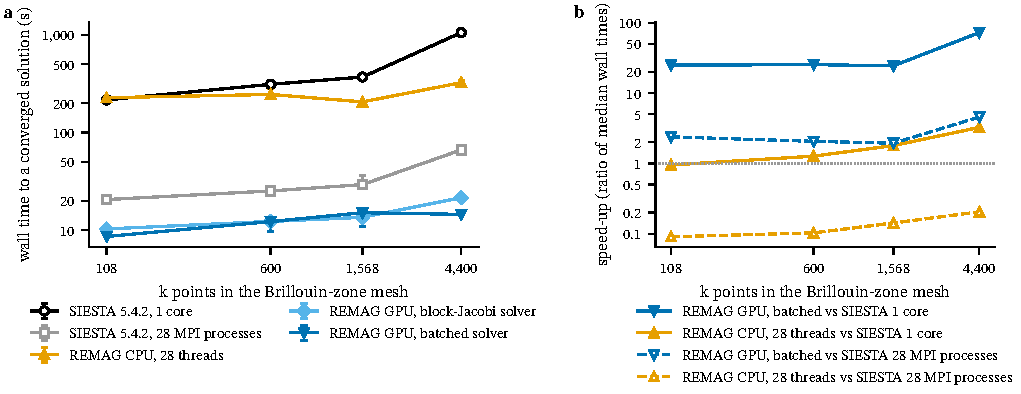
\includegraphics[width=\textwidth]{figures/fig1_scaling.pdf}
\caption{Time to SCF convergence against the number of k points. (a) Wall time of each
configuration: medians of three runs, with bars from the fastest to the slowest. SIESTA on
one CPU was run once on the two largest meshes. (b) Unmodified SIESTA's median time divided
by REMAG's, against SIESTA on one CPU (filled symbols, solid lines) and on 28 MPI processes
(open symbols, dashed lines). Above the dotted line at 1, REMAG is faster.}
\label{fig:scaling}
\end{figure}

With \num{4400} k points, REMAG on the GPU with the batched solver takes \SI{\tBatchedD}{s}
(Figure~\ref{fig:scaling}a). That is \sBatchedMpiD{} times faster than unmodified SIESTA on
28 MPI processes and \sBatchedSerialD{} times faster than SIESTA on one CPU, a figure that
rests on a single one-CPU run. On the three smaller meshes the GPU is \sBatchedMpiC{} to
\sBatchedMpiA{} times faster than MPI SIESTA (Figure~\ref{fig:scaling}b). The ratio jumps
at \num{4400} k points because MPI SIESTA's time more than doubles, from \SI{\tMpiC}{s} to
\SI{\tMpiD}{s}, while the GPU time stays between \SI{\tBatchedA}{s} and
\SI{\tBatchedC}{s} on every mesh. The number of SCF iterations differs between meshes, 17 on
the $14\times14\times8$ mesh against 22 to 24 on the others (Table~\ref{tab:results}). That
is why every curve dips there. On any one mesh, every configuration took the same number of
iterations. The block-Jacobi solver is within two seconds of the batched one up to
\num{1568} k points, and takes \SI{\tBjD}{s} with \num{4400}.

REMAG on 28 CPU threads is slower than MPI SIESTA on every mesh: \SI{\tHostD}{s} against
\SI{\tMpiD}{s} with \num{4400} k points. MPI SIESTA divides the real-space mesh work among
its processes, and REMAG leaves it on one thread. REMAG on the CPU is \sHostSerialD{} times
faster than SIESTA on one CPU with \num{4400} k points, and no faster with \num{108}.

\begin{figure}[t]
\centering
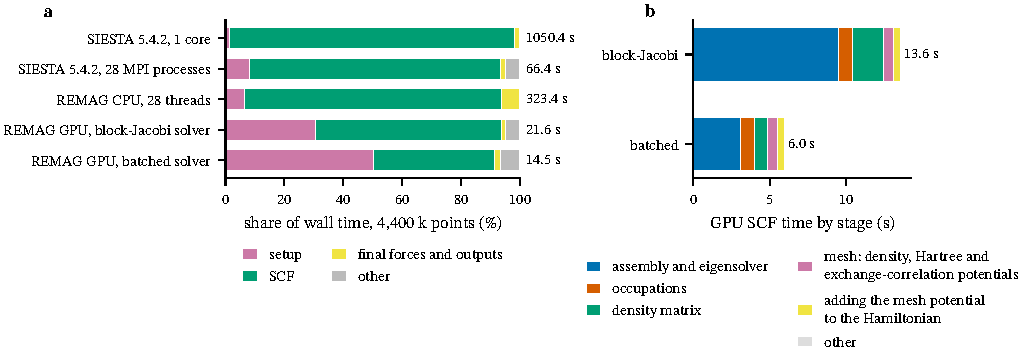
\includegraphics[width=\textwidth]{figures/fig2_breakdown.pdf}
\caption{Where the time goes with \num{4400} k points. (a) The median run of each
configuration divided into setup (basis, neighbour lists, real-space mesh and the first
Hamiltonian), the SCF cycle, and the final forces and output files. ``Other'' is process
start-up and input handling. The total is printed beside each bar. (b) The GPU SCF cycle
divided into its stages. These come from one additional run of each GPU solver in which
the stages ran one after another and were clocked separately.}
\label{fig:breakdown}
\end{figure}

With the batched solver the SCF cycle takes \SI{\scfBatched}{s} of the run, less than the
\SI{\setupBatched}{s} of setup (Figure~\ref{fig:breakdown}a). With the block-Jacobi solver
the SCF cycle is still the largest part, \SI{\scfBj}{s}. For unmodified SIESTA it is nearly
the whole run. The final forces take about \SI{0.3}{s} on the GPU against about \SI{20}{s}
for SIESTA and REMAG on one CPU thread. Setup is shorter for the GPU runs than for REMAG on
the CPU because the first Hamiltonian is built on the GPU. Within the SCF cycle, the batched
solver cuts the time to build and diagonalize the Hamiltonians from \SI{\profBjEig}{s} to
\SI{\profBatchedEig}{s} (Figure~\ref{fig:breakdown}b). Building the density matrix falls
from \SI{\profBjDens}{s} to \SI{\profBatchedDens}{s}, because a whole group of k points is
added into it in one pass instead of one pass per k point.

\begin{figure}[t]
\centering
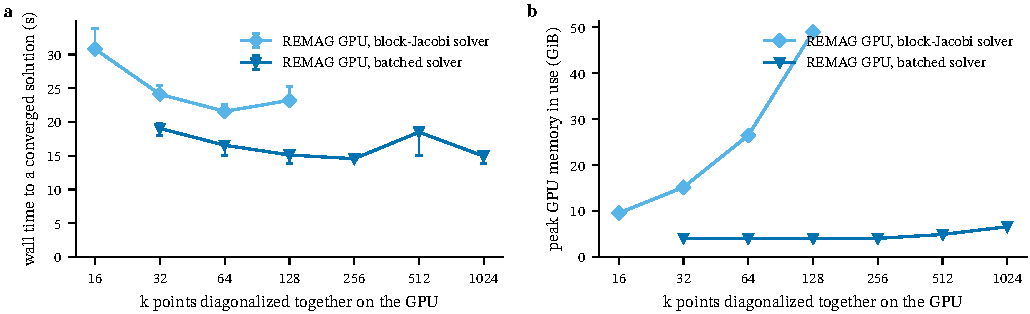
\includegraphics[width=\textwidth]{figures/fig3_batch_width.pdf}
\caption{Effect of the number of k points diagonalized together, with \num{4400} k points
in total. (a) Wall time to SCF convergence, median and range of three runs. (b) Peak GPU
memory in use, read from the driver every \SI{0.25}{s}. The block-Jacobi solver accepts at
most 128 k points at once. Groups of 16 were not run with the batched solver.}
\label{fig:width}
\end{figure}

How many k points are diagonalized together trades speed against memory
(Figure~\ref{fig:width}). The block-Jacobi solver is fastest with 64 at once. Its memory
rises steadily with the group size, from \SI{\mBjSixteen}{GiB} at 16 to
\SI{\mBjOneTwentyEight}{GiB} at 128. The batched solver takes between
\SI{\wBatchedTwoFiftySix}{s} and \SI{\wBatchedOneTwentyEight}{s} with 128, 256 or
\num{1024} at once, and never uses more than \SI{\mBatchedTenTwentyFour}{GiB}. With 512 at
once, two of three runs took about \SI{\wBatchedFiveTwelve}{s}. We did not investigate this.

\begin{figure}[t]
\centering
\begin{minipage}[t]{0.48\textwidth}
\centering
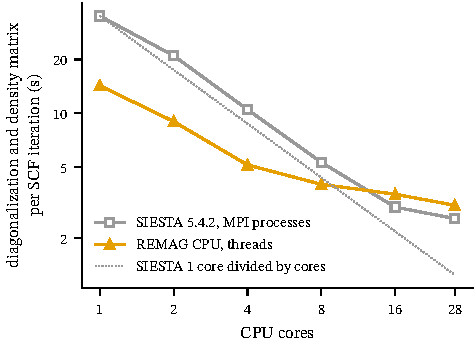
\includegraphics[width=\linewidth]{figures/fig4_cpu_scaling.pdf}
\caption{Wall time per SCF iteration spent diagonalizing the \num{4400} k points and
building the density matrix, against the number of CPUs. The runs stopped after four
iterations. Points are single runs for SIESTA and the mean of two runs for REMAG. The
dotted line is SIESTA on one CPU divided by the number of CPUs. Early iterations cost more
than the average over a full run. For MPI SIESTA on 28 processes, these runs give
\SI{\cMpiTwentyEight}{s} per iteration against \SIrange{1.87}{2.13}{s} in the converged
runs.}
\label{fig:cpuscaling}
\end{minipage}\hfill
\begin{minipage}[t]{0.48\textwidth}
\centering
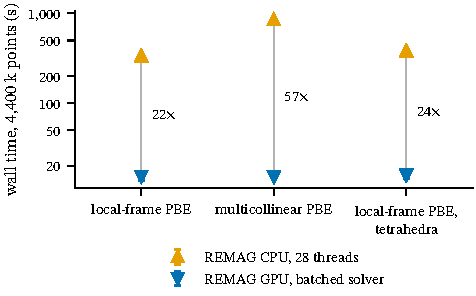
\includegraphics[width=\linewidth]{figures/fig6_methods.pdf}
\caption{Wall time for three treatments that unmodified SIESTA does not offer, with
\num{4400} k points and the moment direction held at \ang{45} from the $c$ axis. Points are
REMAG on 28 CPU threads (one run) and on the GPU with the batched solver (median and range
of three runs). The printed numbers are the ratios.}
\label{fig:methods}
\end{minipage}
\end{figure}

REMAG's CPU threads handle the diagonalizations faster than SIESTA at low CPU counts
(Figure~\ref{fig:cpuscaling}). On one CPU, REMAG takes \SI{\cHostOne}{s} per iteration
against SIESTA's \SI{\cMpiOne}{s}. Most of that gap is SIESTA's second diagonalization of
every k point. REMAG gains little beyond eight threads: \SI{\cHostEight}{s} on 8 and
\SI{\cHostTwentyEight}{s} on 28. MPI SIESTA goes from \SI{\cMpiEight}{s} on 8 processes to
\SI{\cMpiTwentyEight}{s} on 28. That is about twice the ideal value at 28, and it overtakes
REMAG between 8 and 16. We have not measured which part of REMAG's threaded code limits it.

\begin{table}[t]
\centering
\caption{Converged results on each mesh. Every run of every configuration on that mesh
printed exactly these values and took this number of SCF iterations. Energies and the
Fermi level are in eV, and the magnitude of the cell's spin moment is in $\mu_\mathrm{B}$.}
\label{tab:results}
\small
\begin{tabular}{lrrrrrrr}
\toprule
Mesh & k points & Runs & Iterations & Total energy & Free energy & Fermi level & Moment \\
\midrule
$6\times6\times3$ & \num{108} & 15 & 22 & \num{-8326.464264} & \num{-8326.640830} & \num{-5.097158} & \num{3.22154} \\
$10\times10\times6$ & \num{600} & 15 & 23 & \num{-8326.396679} & \num{-8326.603890} & \num{-5.152804} & \num{3.27037} \\
$14\times14\times8$ & \num{1568} & 13 & 17 & \num{-8326.383615} & \num{-8326.598894} & \num{-5.149439} & \num{3.23967} \\
$20\times20\times11$ & \num{4400} & 13 & 24 & \num{-8326.388186} & \num{-8326.600084} & \num{-5.146938} & \num{3.22885} \\
\bottomrule
\end{tabular}

\end{table}

Every configuration produced the same converged state (Table~\ref{tab:results}). This
holds to the last printed digit: \SI{1}{\micro eV} for energies and $10^{-5}\,\mu_\mathrm{B}$
for the moment. The stress tensor also agreed to every printed digit. The forces are zero
by symmetry. The 26 extra runs behind Figures~\ref{fig:breakdown}b and~\ref{fig:width}
gave the same values.

REMAG also runs three treatments that unmodified SIESTA lacks (Figure~\ref{fig:methods}).
In these runs, REMAG's spin constraint, built on the Lagrange-multiplier scheme of
Cuadrado \textit{et al.}~\citep{Cuadrado2018}, holds the moment direction with a field on the
atomic moments. The local-frame form of PBE evaluates the gradient terms of the functional
in the local spin direction at each mesh point, the approach Kübler \textit{et al.}
introduced for the local density approximation~\citep{Kubler1988}. It takes \SI{\methlfBatched}{s} on the GPU
against \SI{\methlfHost}{s} on 28 CPU threads. The multicollinear form of Pu \textit{et al.}~\citep{Pu2023} averages the
collinear functional over 64 spin directions. It takes \SI{\methmcBatched}{s} against
\SI{\methmcHost}{s}. Optimized tetrahedron occupations~\citep{Kawamura2014} replace smearing by an integration
over tetrahedra of k points, with local-frame PBE. They take \SI{\methtetBatched}{s}
against \SI{\methtetHost}{s}. For each treatment the GPU and CPU runs print the same final
energies, Fermi level and moment. With tetrahedra the GPU took 25 iterations and the CPU
28. These ratios compare with REMAG on 28 CPU threads, which is itself about five times
slower than MPI SIESTA on the plain input. They do not measure the GPU against
well-parallelized CPU code.
